
% this file is called up by thesis.tex
% content in this file will be fed into the main document

%: ----------------------- introduction file header -----------------------
\chapter{Preliminaries and geometrical intuition}

%: ----------------------- paths to graphics ------------------------

% change according to folder and file names
\ifpdf
    \graphicspath{{figures/}{figures/}{figures/}}
\else
    \graphicspath{{figures/}{figures/}}
\fi

% ----------------------------------------------------------------------
%: ----------------------- introduction content ----------------------- 
% ----------------------------------------------------------------------
%: ----------------------- HELP: latex document organisation
% the commands below help you to subdivide and organise your thesis
%    \chapter{}       = level 1, top level
%    \section{}       = level 2
%    \subsection{}    = level 3
%    \subsubsection{} = level 4
% note that everything after the percentage sign is hidden from output


\nocite{*}

In this Chapter we introduce some of the ideas which form the foundations of the classical \BN Theory. 
We define the concepts of divisors and line bundles on a curve and, further, the \AJJ map which associates a line bundle to any effective divisor.
Thanks to the Abel's Theorem, this function can be seen as a quotient map and the corresponding equivalence classes are the so called complete linear series, whose behaviour is one of the central themes of the Theory.
Another key ingredient is the famous \RR Theorem which, as we will see, describes the duality between a linear series and its residual one.

All of these concepts are rather abstract, nevertheless we will try to give some insight on their geometrical meaning, by proposing informal interpretations and by taking advantage of some pictures.
We remark that such drawings only represent the real skeleton of the curvem and, therefore, they should not be intended -- in any way -- as precise representations, but just as sketches which may help the reader to build some geometrical intuition.

\section{Divisors and the \AJJ map}

	Let $X$ be a smooth projective curve over an algebraically closed field $k$. Consider the set $\Div_X$ of divisors over $X$ -- i.e. the free abelian group on the points of $X$ -- and denote by $\EDiv_X$ the subset of effective divisors -- i.e. the free monoid on the points of $X$. One can build an intuitive idea of effective divisors by thinking about the finite formal sum $D=\sum_i m_i P_i$ as a \emph{book-keeping device} containing the points of intersection between $X$ and another variety, where the (positive) coefficient $m_i$ of each point $P_i$ measures the multiplicity of the intersection, as Figure \ref{fig:Divisors} shows.

	\begin{figure}[h]
			\centering
			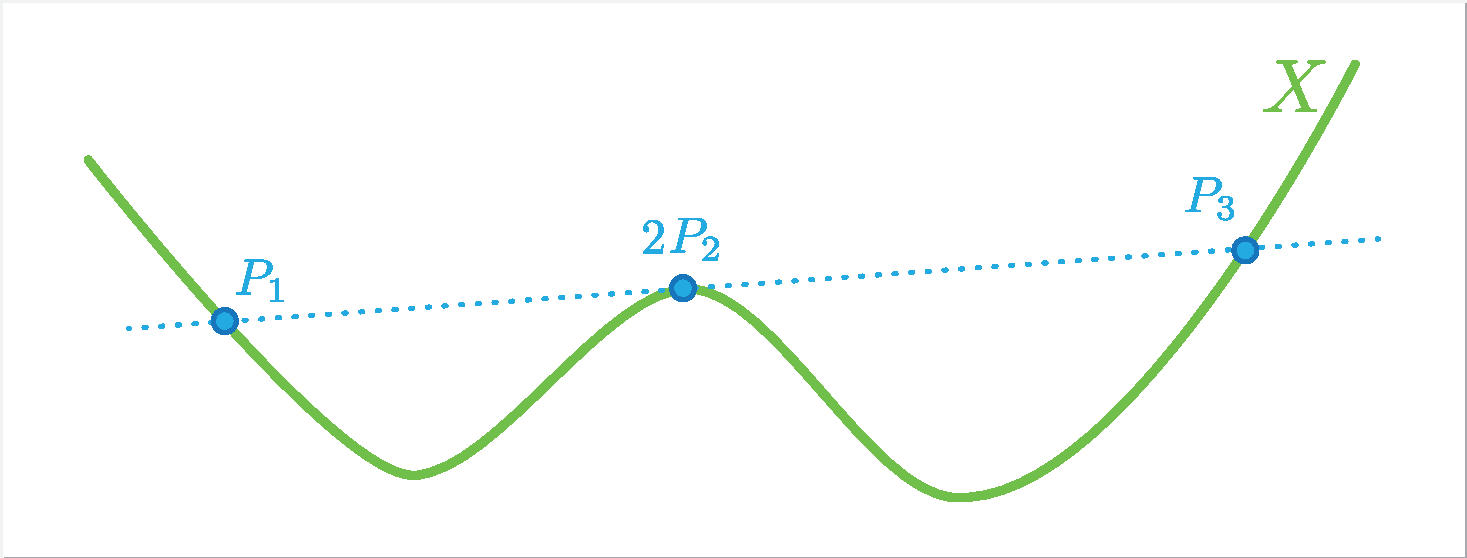
\includegraphics[width=0.9\textwidth]{Divisors.pdf}
			\caption{The effective divisor $P_1 + 2P_2 + P_3$ obtained as the intersection between the curve $X$ and a line}
			\label{fig:Divisors}
	\end{figure}

	Another way to obtain (not necessarily effective) divisors is to start from any non-zero rational map $g$ defined locally on the curve and build a divisor by the recipe
	$$ \Div(g) = (g) = \sum_{P\in X} v_P(g) \cdot P $$
	where $v_P(g)$ is the valuation of $g$ at the point $P$ given by the choice of a local uniformizer. 
	\begin{rema}
		If the divisor of $g$ is given by $(g)=\sum_i m_i P_i$ then, motivated by the definition of \emph{local uniformizer}, we say that on the point $P_i$ the map $g$ presents a \textbf{zero} of order $m_i$ if $m_i>0$, and a \textbf{pole} of order $m_i$ if $m_i<0$.
	\end{rema}	
	Let $f\in k(X)^*$ be globally defined, then the associated divisor $(f)$ is called \textbf{principal divisor} and the well known fact that $\deg(f)=0$ can be explained, informally, by saying that a global rational map on a complete curve has the same number of zeros and poles counted with multiplicity.\\

	The \textbf{degree} of a divisor is defined as the sum of its coefficient, so that it gives a group homomorphism from the set of divisors to $\Z$ and assumes non negative values when restricted to effective divisors. We denote by $\Dd$ the set of effective divisors of degree $d$.\\

	Next, we define the \textbf{Picard group} of $X$ as the sheaf cohomology group
	$$ \Pic_X := H^1(X, \OX^*)\,, $$
	which is well known to be isomorphic to the set of line bundles up to isomorphism, with group structure induced by the usual tensor product of coherent sheaves. 

	To any divisor $D\in \Div_X$ one can associate the line bundle $\OXD$ defined over any open set $U\subset X$ by the prescription
	$$ H^0(U, \OXD) = \left\{\; f \in k(X)^* \mid (f)_{\mid U} + D_{\mid U} \geq 0 \;\right\} $$
	which can be seen as the line bundle whose global sections are locally controlled by $D$. 
	In other words, the sections of $\OXD$ are allowed to present poles on any point of the support of $D$, with order bounded by the coefficient of the point appearing in the formal sum. \\
	It is an easy consequence of the \RR Theorem that every line bundle $L$ on $X$ admits a global section $s$ and, thus, it can be written in the form $L=\OX(D)$ with $D=(s)$ being the divisor corresponding to such a section. Thus we define the \textbf{degree} of $L$ to be the degree of the divisor $D$. We will denote by $\Pd$ the set of line bundles of degree $d$.
	\\
	Based on the above construction, we give a definition of the so called \textbf{\AJJ map} by the assignment
	$$ u: \Div_X\to\Pic_X \qquad D\mapsto \OXD $$ 
	\begin{rema}
		Recall that classically, in the theory of smooth curves over $\C$, the \AJJ map is defined for a one-point divisor $P$ (and then extended linearly) by means of the Abelian integrals as
		$$ u:X_d \to J(X), \qquad P \mapsto \left(\; \int_{P_0}^{P} \omega_1 \;,\; \dots\;,\; \int_{P_0}^{P} \omega_g \;\right) \mod \Lambda, $$
		where $P_0$ is a fixed point of $X$, the $\w_i$'s form a basis of the space of Abelian differentials and $\Lambda$ is a nondegenerate lattice arising from the Riemann bilinear relations.\\
		Our definition of the \AJJ map is simpler, more elegant and does not rely on analytical tools such as path-integration, nevertheless it turns out to be equivalent to its classical counterpart.
	\end{rema}


\section{Linear equivalence and Abel's Theorem}

	Principal divisors can be used to define an equivalence relation on the set of divisors of $X$, by declaring two divisors $D$ and $E$ to be \textbf{linearly equivalent} if they differ by a principal divisor. More precisely, we define
	$$ D\sim E \;\overset{\text{def}}\iff\; \exists\; f \in k(X)^* \text{ such that } E = D + (f) $$
	and, given an effective divisor $D\in \EDiv_X$, we denote by $|D|$ the set of all effective divisors which are linearly equivalent to $D$, the so called \textbf{complete linear series} of $D$.\\
	By sending a global section $f\in H^0(D)$ to the divisor $(f)+D$, we obtain a canonical isomorphism
	$$ \PP H^0(D) \;\cong\; |D| $$
	which identifies the complete linear series of $D$ with the projectification of the vector space of global sections of the line bundle $\OXD$. Motivated by this observation, to any linear subspace $V\subset H^0(D)$ we associate the projective space $\PP V$ and call it a (not necessarily complete) \textbf{linear series}.
	\begin{defi}
		Let $D$ be a divisor of degree $d$ and $V\subset H^0(D)$ a linear subspace of dimension $r+1$. We define a $g_d^r$ to be the linear series associated to $\PP V$.
	\end{defi}

	The classical Abel's Theorem states that the quotient map associated to the equivalence relation defined above is nothing but the \AJJ map or, in other terms, that the fibres of $u$ are complete linear series.
	\begin{namedtheo}[Abel's Theorem]\label{thm:Abel}
		Let $D,E \in \EDiv_X$ be two effective divisors of degree $d$ on $X$. Then
		$$ D\sim E \iff u(D) = u(E). $$
	\end{namedtheo}
	Abel's Theorem was originally proved for Riemann surfaces -- see \cite{GAC} for instance -- but it remains valid for smooth curves over of any algebraically closed field. It plays a crucial role in the \BN theory because it allows to treat linear series as degeneracy loci of the \AJJ map, as we will see in Section \ref{sec:fitt_deg}.
	

\section{The canonical map}

	The recipe we used to obtain divisor $(g)$ from a locally defined rational map $g$ can be extended to the define divisor associated to sections of arbitrary line bundles. In particular, given any global section $\w$ of the cotangent bundle of $X$, we can pick an open cover $\bigcup_i U_i$ of $X$ and a local uniformizer $\pi_i$ for every $U_i$, then $\w$ can be written locally on every $U_i$ as $\w = g_i \; d\,\pi_i$ and the corresponding divisor $(\w) := \sum_i (g_i)$ is called \textbf{canonical divisor}.
	\begin{rema}
		All the canonical divisors on a curve of genus $g$ are linearly equivalent and, as it follows from the \RR Theorem, have degree $2g-2$. Notice that, if $g>0$, a canonical divisor is not principal and its degree is non-zero.
	\end{rema}
	\begin{notation}
		From now on we will abuse notation and write $K$ both for any canonical divisor and for the cotangent bundle $\Omega_X^1$, while the corresponding cohomology groups will be denoted by $H^i(K)$.
	\end{notation}
	
	Next, recall the definition of a base-point-free linear series which we will need for the following construction.
	\begin{defi}
		A $g_d^r$ is said to be \textbf{base-point-free} if there is no point which is contained in the supports of all the divisors belonging to the linear series.
	\end{defi}
	Any base-point-free $g_d^r$ with linear series $\PP V$ can be used to obtain a map of the curve $X$ to a projective space, by considering the assignment
	$$ \phi_V : X\to \PP V^{*} \qquad P\mapsto \set{ s\in V \mid s(P)=0 } \,.$$
	Notice that, since the $g_d^r$ is base-point-free, the requirement $s(P)=0$ gives a non trivial linear condition hence it defines an hyperplane of $V$. Therefore $\phi_V(P)$ can be seen as a point of the dual projective space $\PP V^*$ parametrizing hyperplanes and, thus, $\phi_V$ is a well-defined function.

	\begin{defi}
		We extend the map $\phi_V$ to any effective divisor $D=\sum_{i=1}^d P_i$ with distinct points, by declaring $ \phi_V(D) := \operatorname{span}\{\phi_V(P_1), \dots, \phi_V(P_d)\}$.
	\end{defi}	

	Let us now assume that $X$ has genus $g\geq 2$. Choose any canonical divisor $K$ and recall that the \textbf{genus} of $X$ is defined as $g:=h^0(X, K)$, so that the complete linear series $|K|$ gives rise to a map $\phi_K : X \to \PP^{g-1}$ which is called the \textbf{canonical map}. \\
	It is easy to show that, if $X$ is not hyperelliptic, this map is in fact an embedding and gives a canonical, preferred realization of our curve in a $(g-1)$-dimensional projective space. If the curve is hyperelliptic, instead, $\phi_K:X\to \PP^{g-1}$ is not an embedding, but a $2$ to $1$ map exhibiting $X$ as a double cover of a rational normal curve in $\PP^{g-1}$.
	\begin{figure}[H]
  	\centering
    \begin{subfigure}[b]{0.3\textwidth}
        \centering
					\begin{tikzpicture}[node distance=3.5em, auto]
					\node (X) 									{$X$};
					\node (SP) 	[right of=X]		{$\;$};
				  \node (PP) 	[right of=SP] 	{$\PP^{g-1}$};
				  \node (P1) 	[below of=SP] 	{$\;$};
				  \draw[-stealth, right hook-stealth] 	(X) to node 	{$\phi_K$}				(PP);
				\end{tikzpicture}	  	
      \caption{$X$ not hyperelliptic}
      \label{fig:not_hyp}
    \end{subfigure}
    \qquad
    \begin{subfigure}[b]{0.3\textwidth}
        \centering
					\begin{tikzpicture}[node distance=3.5em, auto]
					\node (X) 									{$X$};
					\node (SP) 	[right of=X]		{$\;$};
				  \node (PP) 	[right of=SP] 	{$\PP^{g-1}$};
				  \node (P1) 	[below of=SP] 	{$\PP^1$};
				  \draw[-stealth] 									(X) to node 	{$\phi_K$}				(PP);
				  \draw[-stealth][swap] 						(X) to node 	{$h$} 					(P1);
				  \draw[right hook-stealth][swap] (P1) to node	{$v_{g-1}$}			(PP);
				\end{tikzpicture}	  	
      \caption{$X$ hyperelliptic}
      \label{fig:hyp}
    \end{subfigure}
	\end{figure}
	
	\begin{assumption}
		For the rest of the Chapter we will assume that $X$ is not hyperelliptic and, for simplicity, we identify $X$ with its isomorphic image $\phi_K(X)$.
	\end{assumption}	

	The most interesting feature of the canonical embedding is that, by construction, any global section of the cotangent bundle $\w\in H^0(X,K)$ corresponds to a hyperplane $H_{\w}\,\subset\,\PP^{g-1}$ which intersects $X$ precisely in the points forming the support of the divisor $(\w)$, counted with the right multiplicity.

	\begin{figure}[h]
		\centering
		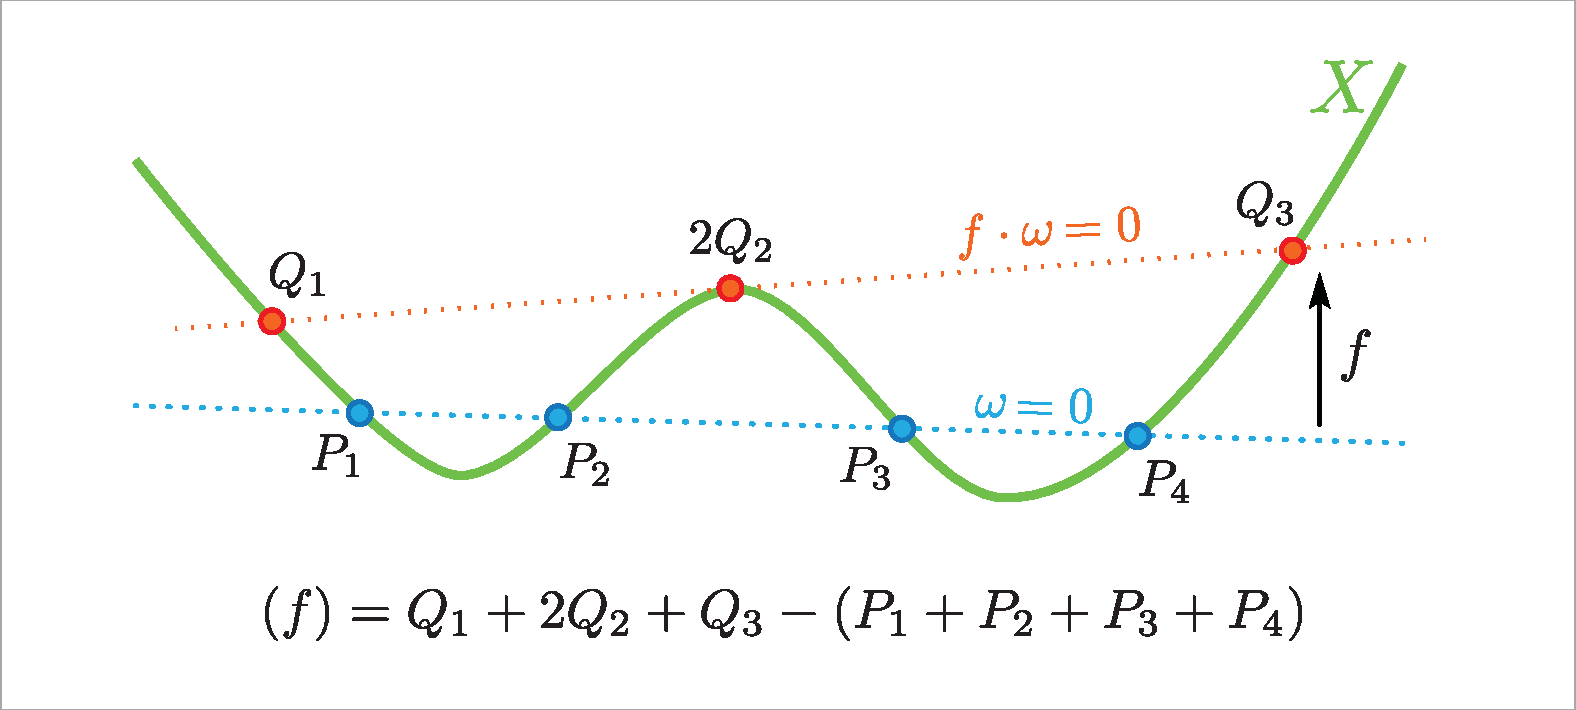
\includegraphics[width=0.9\textwidth]{canonical_embedding_new.pdf}
		\caption{The canonical embedding of a non-hyperelliptic curve of genus $g=3$ in the plane. The picture shows how two canonical divisors are linearly equivalent, being connected by a moving hyperplane }
		\label{fig:canonical_embedding}
	\end{figure}

	Given any rational map $f\in k(X)$, the product $f\cdot \w$ is still an element of $H^0(X,K)$ and, therefore, it corresponds to another hyperplane $H_{f\w}$ via the canonical embedding. Since the support of $(f\cdot\w) = (f)+(\w)$ is in general different from the one of $(\w)$, we can interpret $f$ geometrically as a transformation which \emph{moves} the hyperplane $H_\w$ to a different hyperplane $H_{f\w}$.
	Hence we could informally say that, under the canonical embedding, two divisors are linearly equivalent \ABiff \emph{they are connected by a moving hyperplane}. \\

	This intuitive idea is pictured in Figure \ref{fig:canonical_embedding}, where an non-hyperelliptic curve of genus $g=3$ is considered, so that $\phi_K$ embeds it into $\PP^2$. Notice that, in this example, the linearly equivalent divisors $P_1+P_2+P_3+P_4$ and $Q_1+2Q_2+Q_3$ are both canonical and have degree $2g-2 = 4$.


\section{The \RR Theorem}

	Given any divisor $D$ on $X$, define its \textbf{residual divisor} or \textbf{dual divisor} as $D' := K-D$. Looking at the canonical embedding of our non hyperelliptic curve and considering a divisor $D$ of degree $d<g$ consisting distinct points, we claim that we can always find a canonical divisor $K=(\w)$ such that $D\leq K$. Indeed, we can always find a hyperplane of $\PP^{g-1}$ passing through the $\phi_K(D)$, whose dimension is at most $d-1$.
	In this setting we can think of the support of the residual $D'$ as those points of intersection between the hyperplane and the curve which do not belong to the support of $D$ -- see Figure \ref{fig:Duality}.\\

	\begin{figure}[ht]
			\centering
			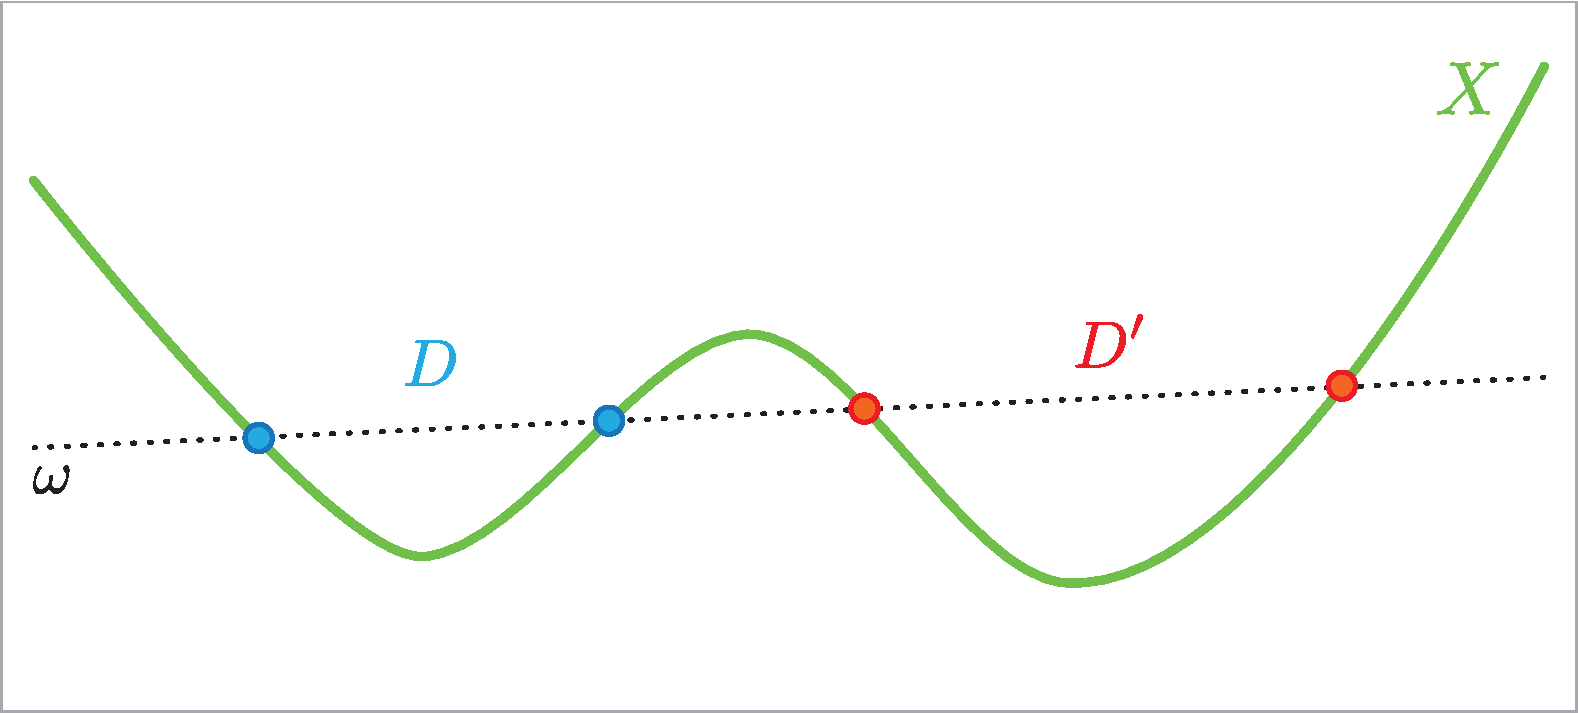
\includegraphics[width=\textwidth]{Duality.pdf}
			\caption{A divisor $D$ of degree $d=2$ and its residual, pictured in the canonical embedding of a genus $3$ curve. In this particular case, since $\deg(\w)=2g-2=4$, the degree $d'$ of the residual divisor is $2$, as well }
			\label{fig:Duality}
	\end{figure}

	The famous \RR Theorem \ref{thm:RR} can be interpreted, thanks to Serre duality, as a statement on the relationship between a divisor and its residual. In fact, given a divisor $D\in \Div_X$ of degree $d$, the \RR formula
	$$ h^0(D) - h^0(D') = d-g+1 $$
	implies that the knowledge of the dimension of $H^0(D)$ is equivalent to that of the dimension of $H^0(D')$ and viceversa.\\

	We highlight, moreover, that the statement of the \RR is completely symmetric with respect to residual duality. Indeed, since the degree of the canonical divisor equals $2g-2$ and the degree of $D'$ is given by $d' = \deg(K)-d$, one can easily see that a completely equivalent formulation of the Theorem is
	$$ h^0(D') - h^0(D) = d'-g+1 $$
	thus showing that the \RR does not discriminate between a divisor and its residual. This implies that the information we can get from the behaviour of a given divisor can be equivalently obtained by looking at its residual and viceversa, a fact which will be exploited to draw Figure \ref{fig:Exceptional_Divisors}.\\

	The relationship between the Theorem and linear series is therefore well understood by means of the above mentioned canonical isomorphism
	$ \PP H^0(D) \;\cong\; |D| $
	which identifies the complete linear series of $D$ with the projectification of the space of global sections of $\OXD$. Therefore, using the standard notation $r(D):= \dim|D| $ for the dimension of $|D|$, we can rewrite the \RR formula as
	\begin{equation}\label{eq:RR}
		r(D') - r(D) = d'-g+1
	\end{equation}
	thus making it clear that it can be interpreted as a statement on the \emph{dimension spread} between a linear series and its residual.\\

	The \RR Theorem is an extremely useful result, with applications ranging from pure mathematics to applied graph theory and even communication engineering. But what is the geometrical meaning of the Riemann-Roch formula? We will try to answer this fascinating question in the following Sections.
	

\section{Special exceptional divisors}\label{sec:special}

	Some divisors on the curve $X$ -- and the corresponding linear series -- are \emph{more important} than others, in the sense that they contain more information about the curve itself.\\ 
	A good reason to study the so called \textbf{special exceptional divisors} of a given curve, as we will exemplify in Section \ref{sec:examples}, is that the behaviour of the corresponding linear series may help distinguish the curve among other curves.\\
	Put $r=r(D)$. For a curve of genus $g$ the region of special exceptional divisors is given, as a subset of the $(d,r)$-plane, by the inequalities
	$$ r>0 \AND 2r<d<g $$ 
	as we picture in Figure \ref{fig:Exceptional_Divisors}. The reasons for these constraints are the following:
	\begin{itemize}
		\item If $r=0$ then the linear series $|D|$ is trivial;
		\item Due to the duality involved in the \RR formula, we can restrict our attention to linear series of degree $d<g$;
		\item For non trivial linear series of degree $d<g$, Clifford's Theorem \ref{thm:Clifford} gives the upper bound $r<d/2$.
	\end{itemize}

	\begin{figure}[ht]
		\centering
		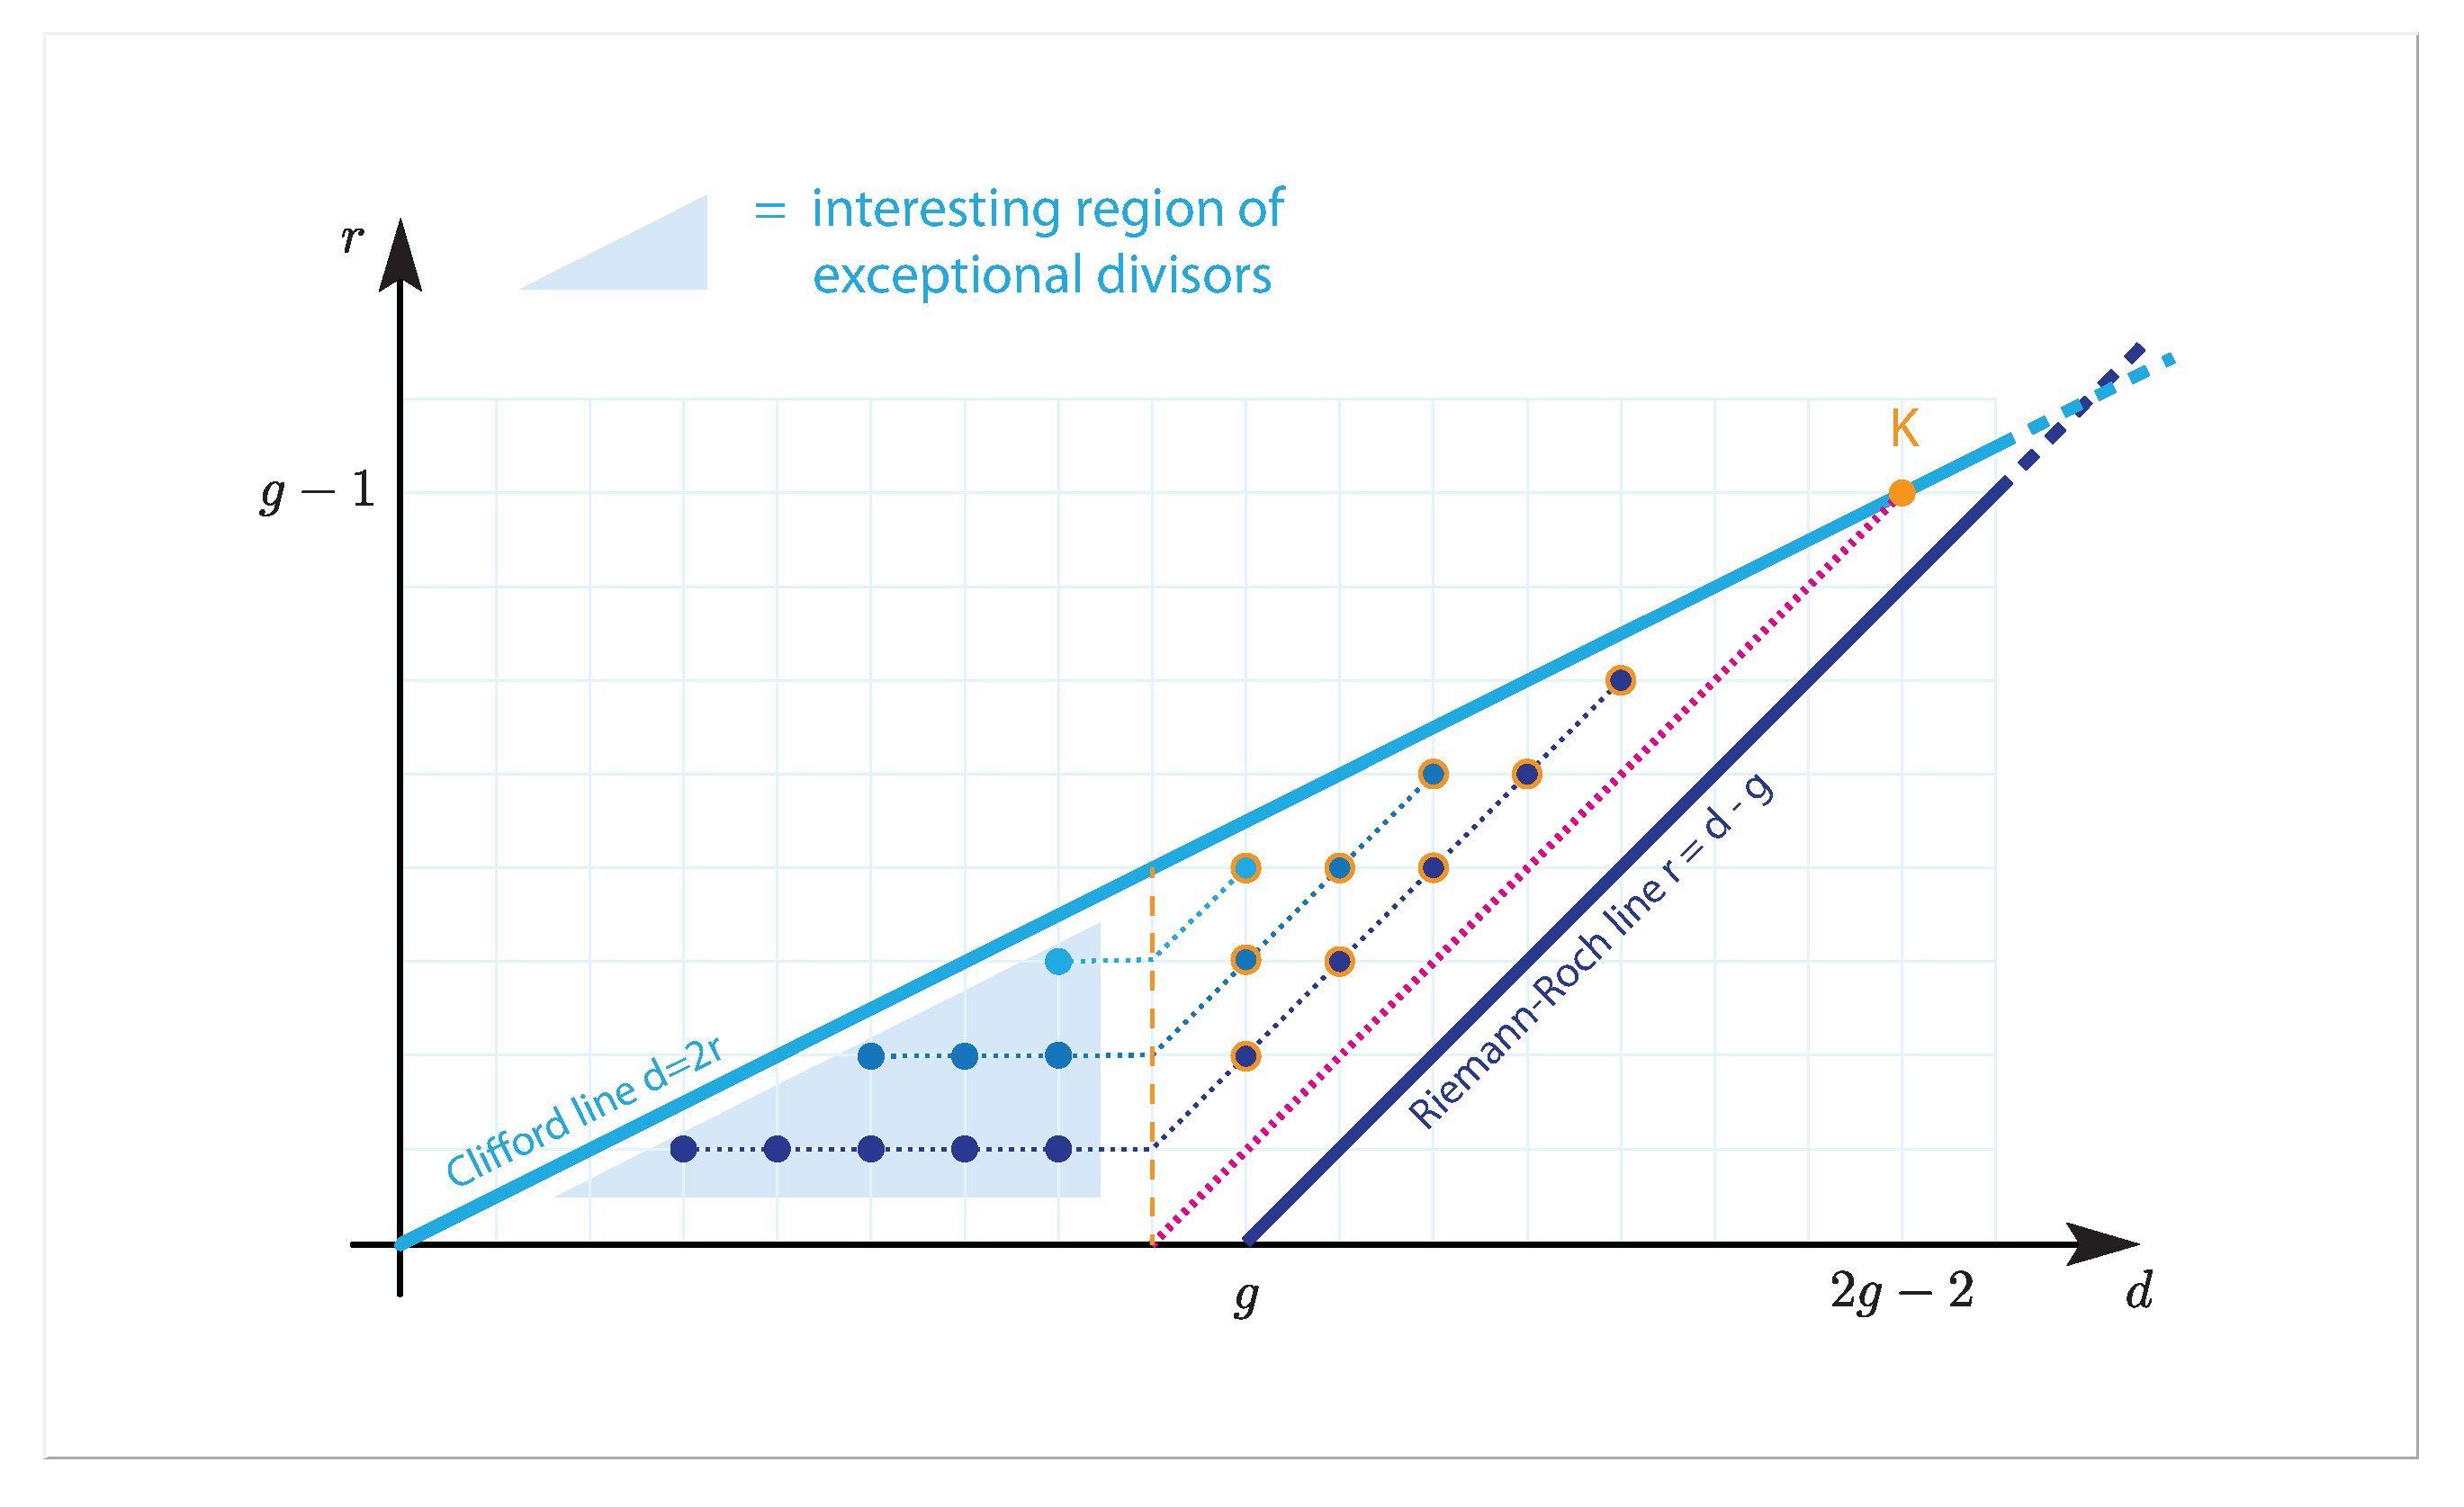
\includegraphics[width=0.85\textwidth]{Exceptional_Divisors_new.pdf}
		\caption{ The region of Special Exceptional divisors for a curve of genus $g=9$ }
		\label{fig:Exceptional_Divisors}
	\end{figure}


\section{Geometrical interpretation}

	In the following we will give some insights into the geometrical meaning of the \RR formula. In order to do so, we start by introducing the cup-product map
	$$ \mu_0: H^0(D)\otimes H^0(K-D) \tolong H^0(K) $$ 
	which is also know as the \textbf{Petri's map} and, as we will see in Chapter \ref{chap:moduli}, plays a fundamental role in the linear approximation of the varieties \moduu parametrizing linear series.\\

	Consider an effective divisor $D$ of degree $d<g$ consisting of distinct points and notice that the vector space $H^0(K-D)$ can be interpreted as the linear subspace consisting of those $\w\in H^0(K)$ such that $(\w)\geq K$ or, in other words, $\PP H^0(K-D)$ parametrizes the hyperplanes of $\PP^{g-1}$ which cut $X$ in a set of points containing $D$. Among these hyperplanes there is a unique one passing through the support of the residual $D'$, which can be identified with the unique generator of $H^0(K-D-D')\cong H^0(\OX)$.\\ 
	Now, by restricting the Petri's map to $H^0(D)\otimes H^0(K-D-D')$, we get a map
	$$ \mu_0: H^0(D)\otimes H^0(K-D-D') \tolong H^0(K-D') $$
	whose target space corresponds (up to scalar multiplication) to the hyperplanes cutting the curve in a set of points containing the support of $D'$. From the natural isomorphism $H^0(K-D')\cong H^0(D)$ we deduce that the number of such hyperplanes is given by the integer $r(D) = \dim \PP H^0(D)$, a fact which can be used to shade light on the geometrical interpretation of the \RR. Indeed, one can equivalently rewrite the formula \eqref{eq:RR} as
	$$ r(D) = [\;g-1\;] \; - \; [\;d'-r(D')\;] $$
	and observe that $g-1$ is nothing but the dimension of the projective space $\PP^{g-1}$ in which $X$ is canonically embedded. Therefore we see that $d'-r(D')$ equals the number of linearly independent points of the support of $D'$ and, consequently, that the integer $r(D')$ counts the number of independent linear relations among these points. Hence the \RR is \emph{simply} telling us that the complete linear series $|D|$ can be geometrically visualized as a family of hyperplanes passing through $\phi_K(D')$, each one of them cutting $X$ in a set of points consisting of $D'$ plus a divisor in $|D|$.

	Therefore we understand how the fact that the \emph{dimension spread} $r(D)-r(D')$ is a constant depending on $d$ and $g$ has a clear geometrical meaning: a higher number $r(D')$ of independent linear relations among the support of $D'$ corresponds to a larger family of hyperplanes passing through $\phi_K(D')$, the dimension of this family being precisely the dimension $r(D)$ of the linear series $|D|$.\\  

	In the next page, we show two pictures that might help the reader visualizing the geometrical meaning of $r(D)$, in the context of the canonical embedding of a curve of genus $4$. Figure \ref{fig:Example} presents an example of a $g_1^3$, whit one linear relation among the $3$ points of $D$, while Figure \ref{fig:Example2} shows a trivial linear series, where no linear relations among the points of $D$ is present.\\

	Moreover, notice that the above geometrical interpretation allows to exclude some otherwise possible scenarios. For instance, the canonical embedding of a genus $4$ curve cannot appear as pictured in Figure \ref{fig:Impossible}, because this would correspond to the values $d=2$, $d'=4$ and $r(D)=0$, $r(D')=2$ which do not satisfy the \RR formula.
	\vspace{1.5em}
	\begin{figure}[H]
		\centering
		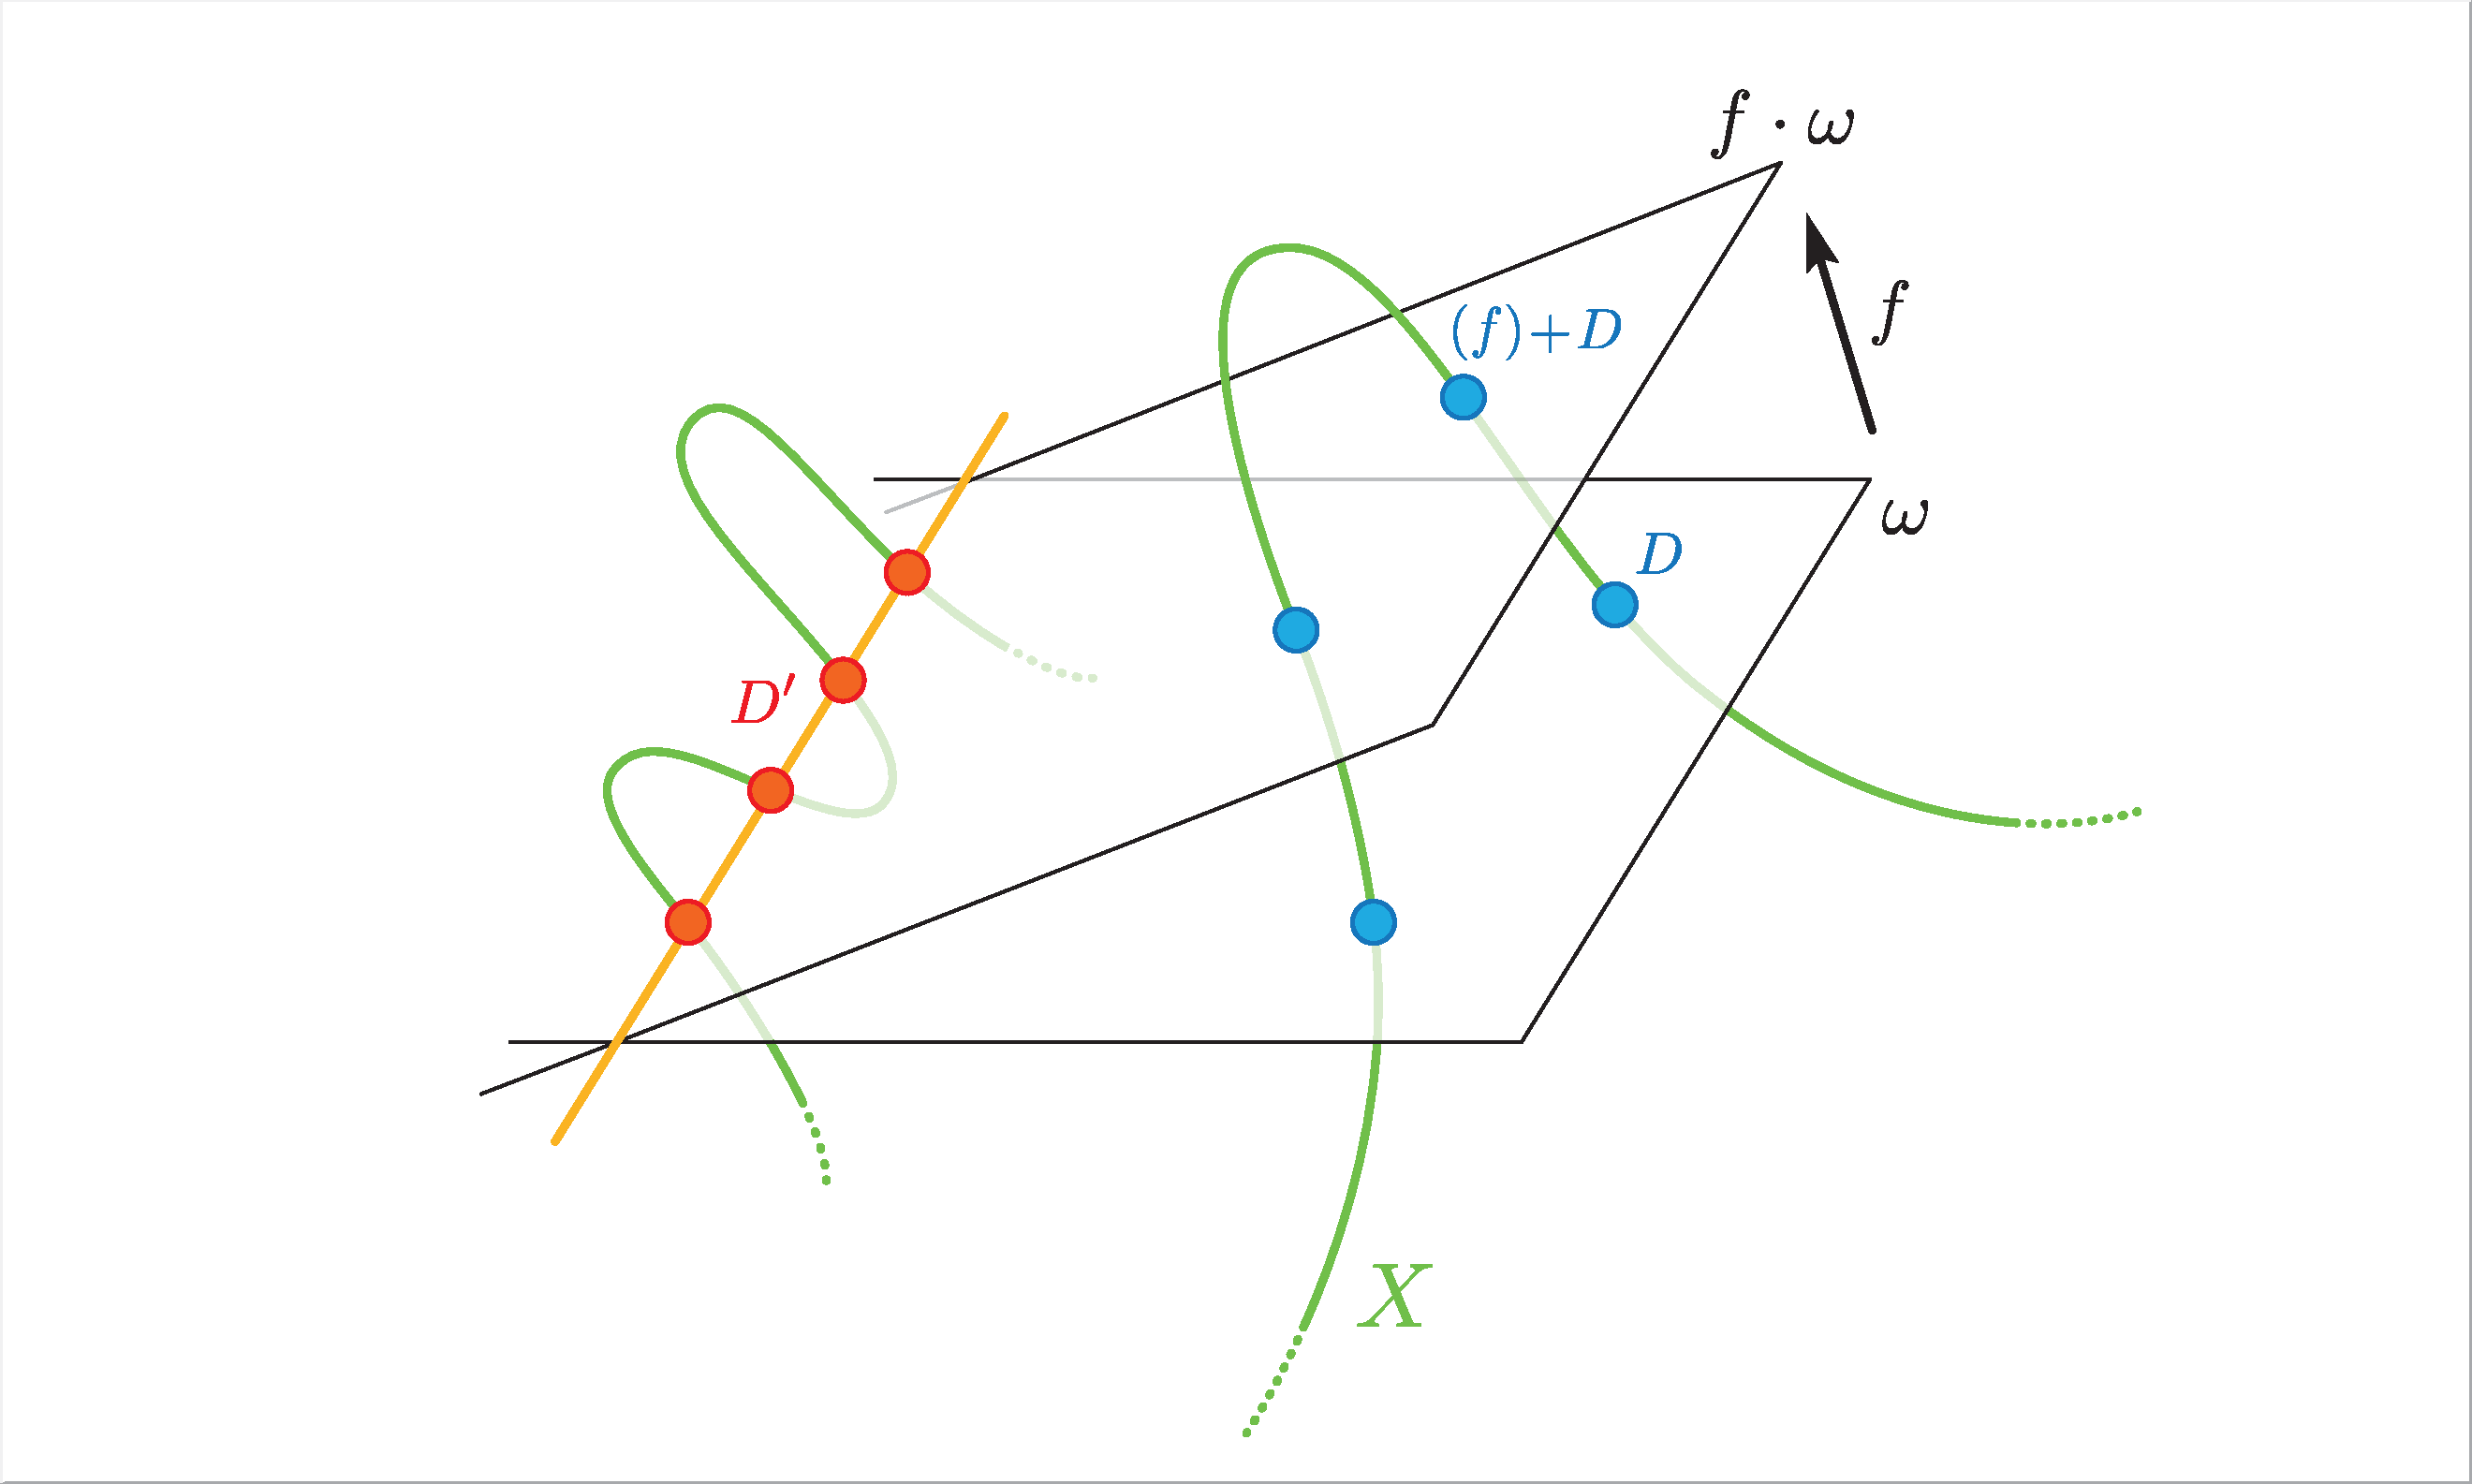
\includegraphics[width=0.85\textwidth]{Impossible.pdf}
		\caption{An hypothetical curve of genus $4$ embedded in $\PP^3$, showing a $g_2^0$ whose residual series is a $g_4^2$. This situation is actually impossible, as one can deduce form the \RR Theorem }
		\label{fig:Impossible}
	\end{figure}

	%in the context of the canonical embedding of a curve of genus $4$\newpage

	\begin{figure}[H]
		\centering
		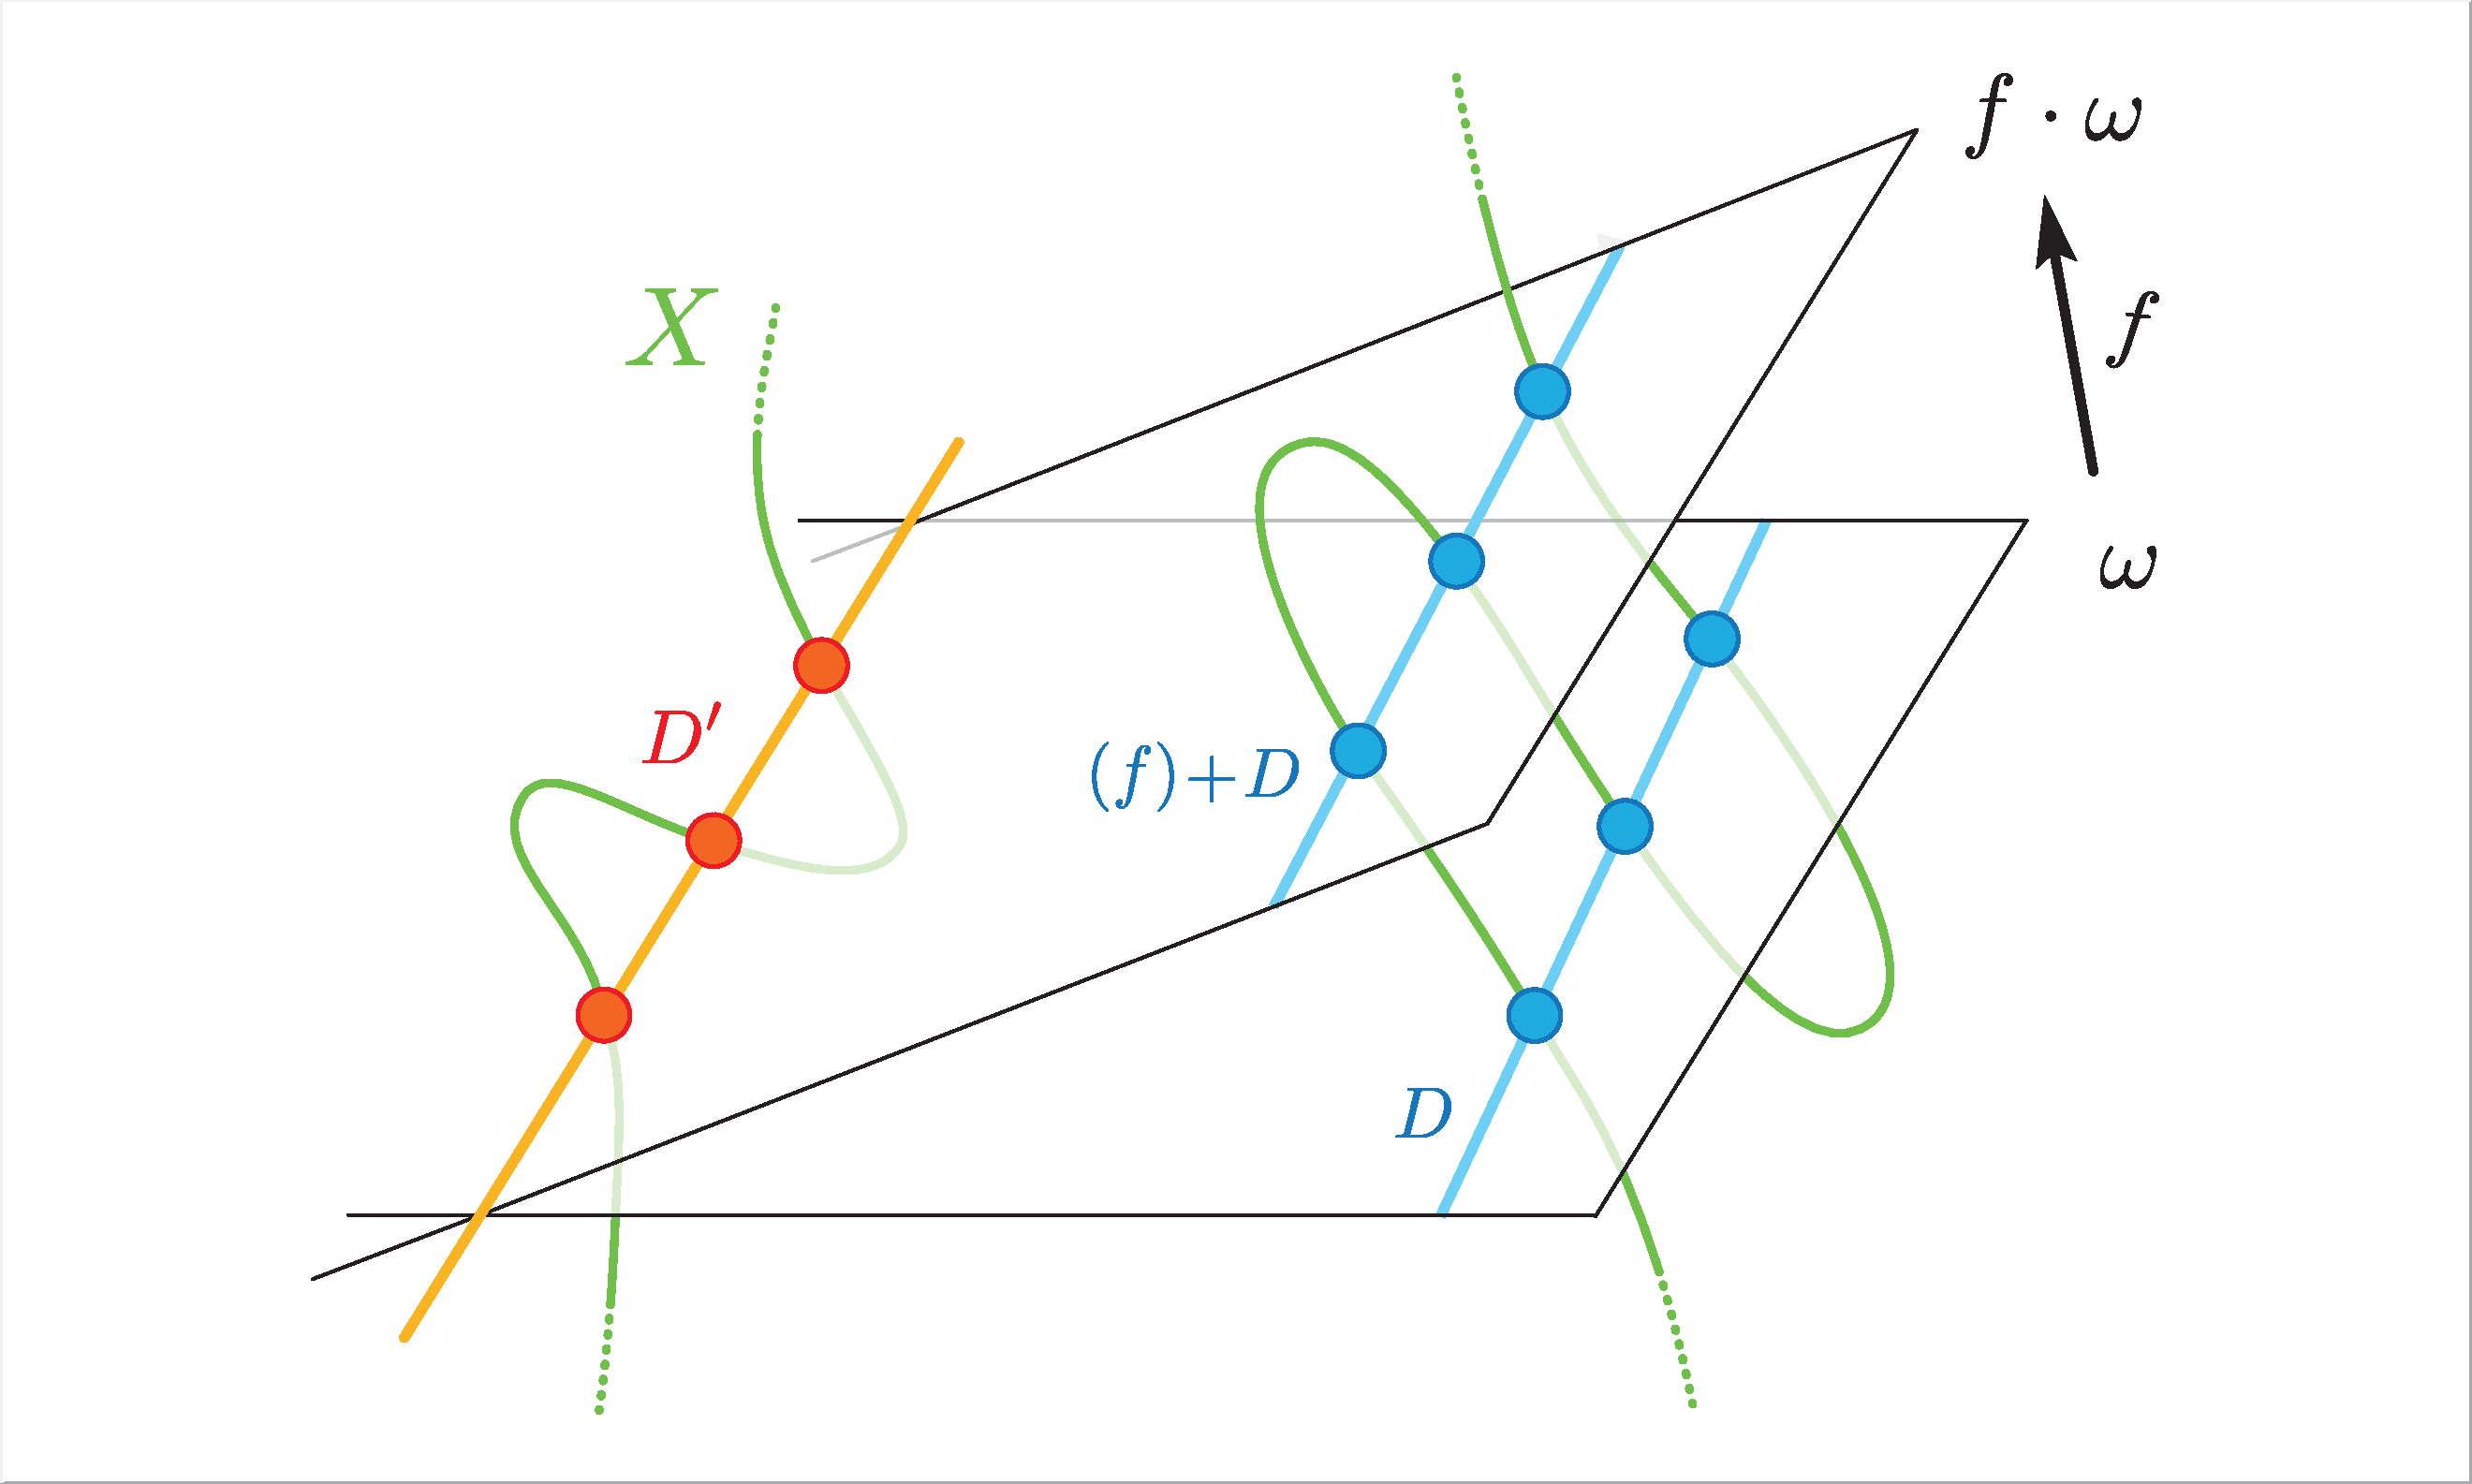
\includegraphics[width=0.85\textwidth]{Example.pdf}
		\caption{An example of a complete linear series on a curve of genus $4$ canonically embedded into $\PP^3$. The global section $f\in H^0(D)$ has poles only on the points of $D$, hence the hyperplane $H_{\w}$ associated to $\w \in H^0(K-D-D')$ is moved away from $D$ by $f$, but stays on the points of the residual divisor $D'$. Notice that, for this particular choice of $D$, there is one linear relation among the points of both $D$ and $D'$, so that $r(D)=r(D')=1$ and each divisor gives rise to a $g_3^1$. }
		\label{fig:Example}
		
		\vspace{4em}

		\centering
		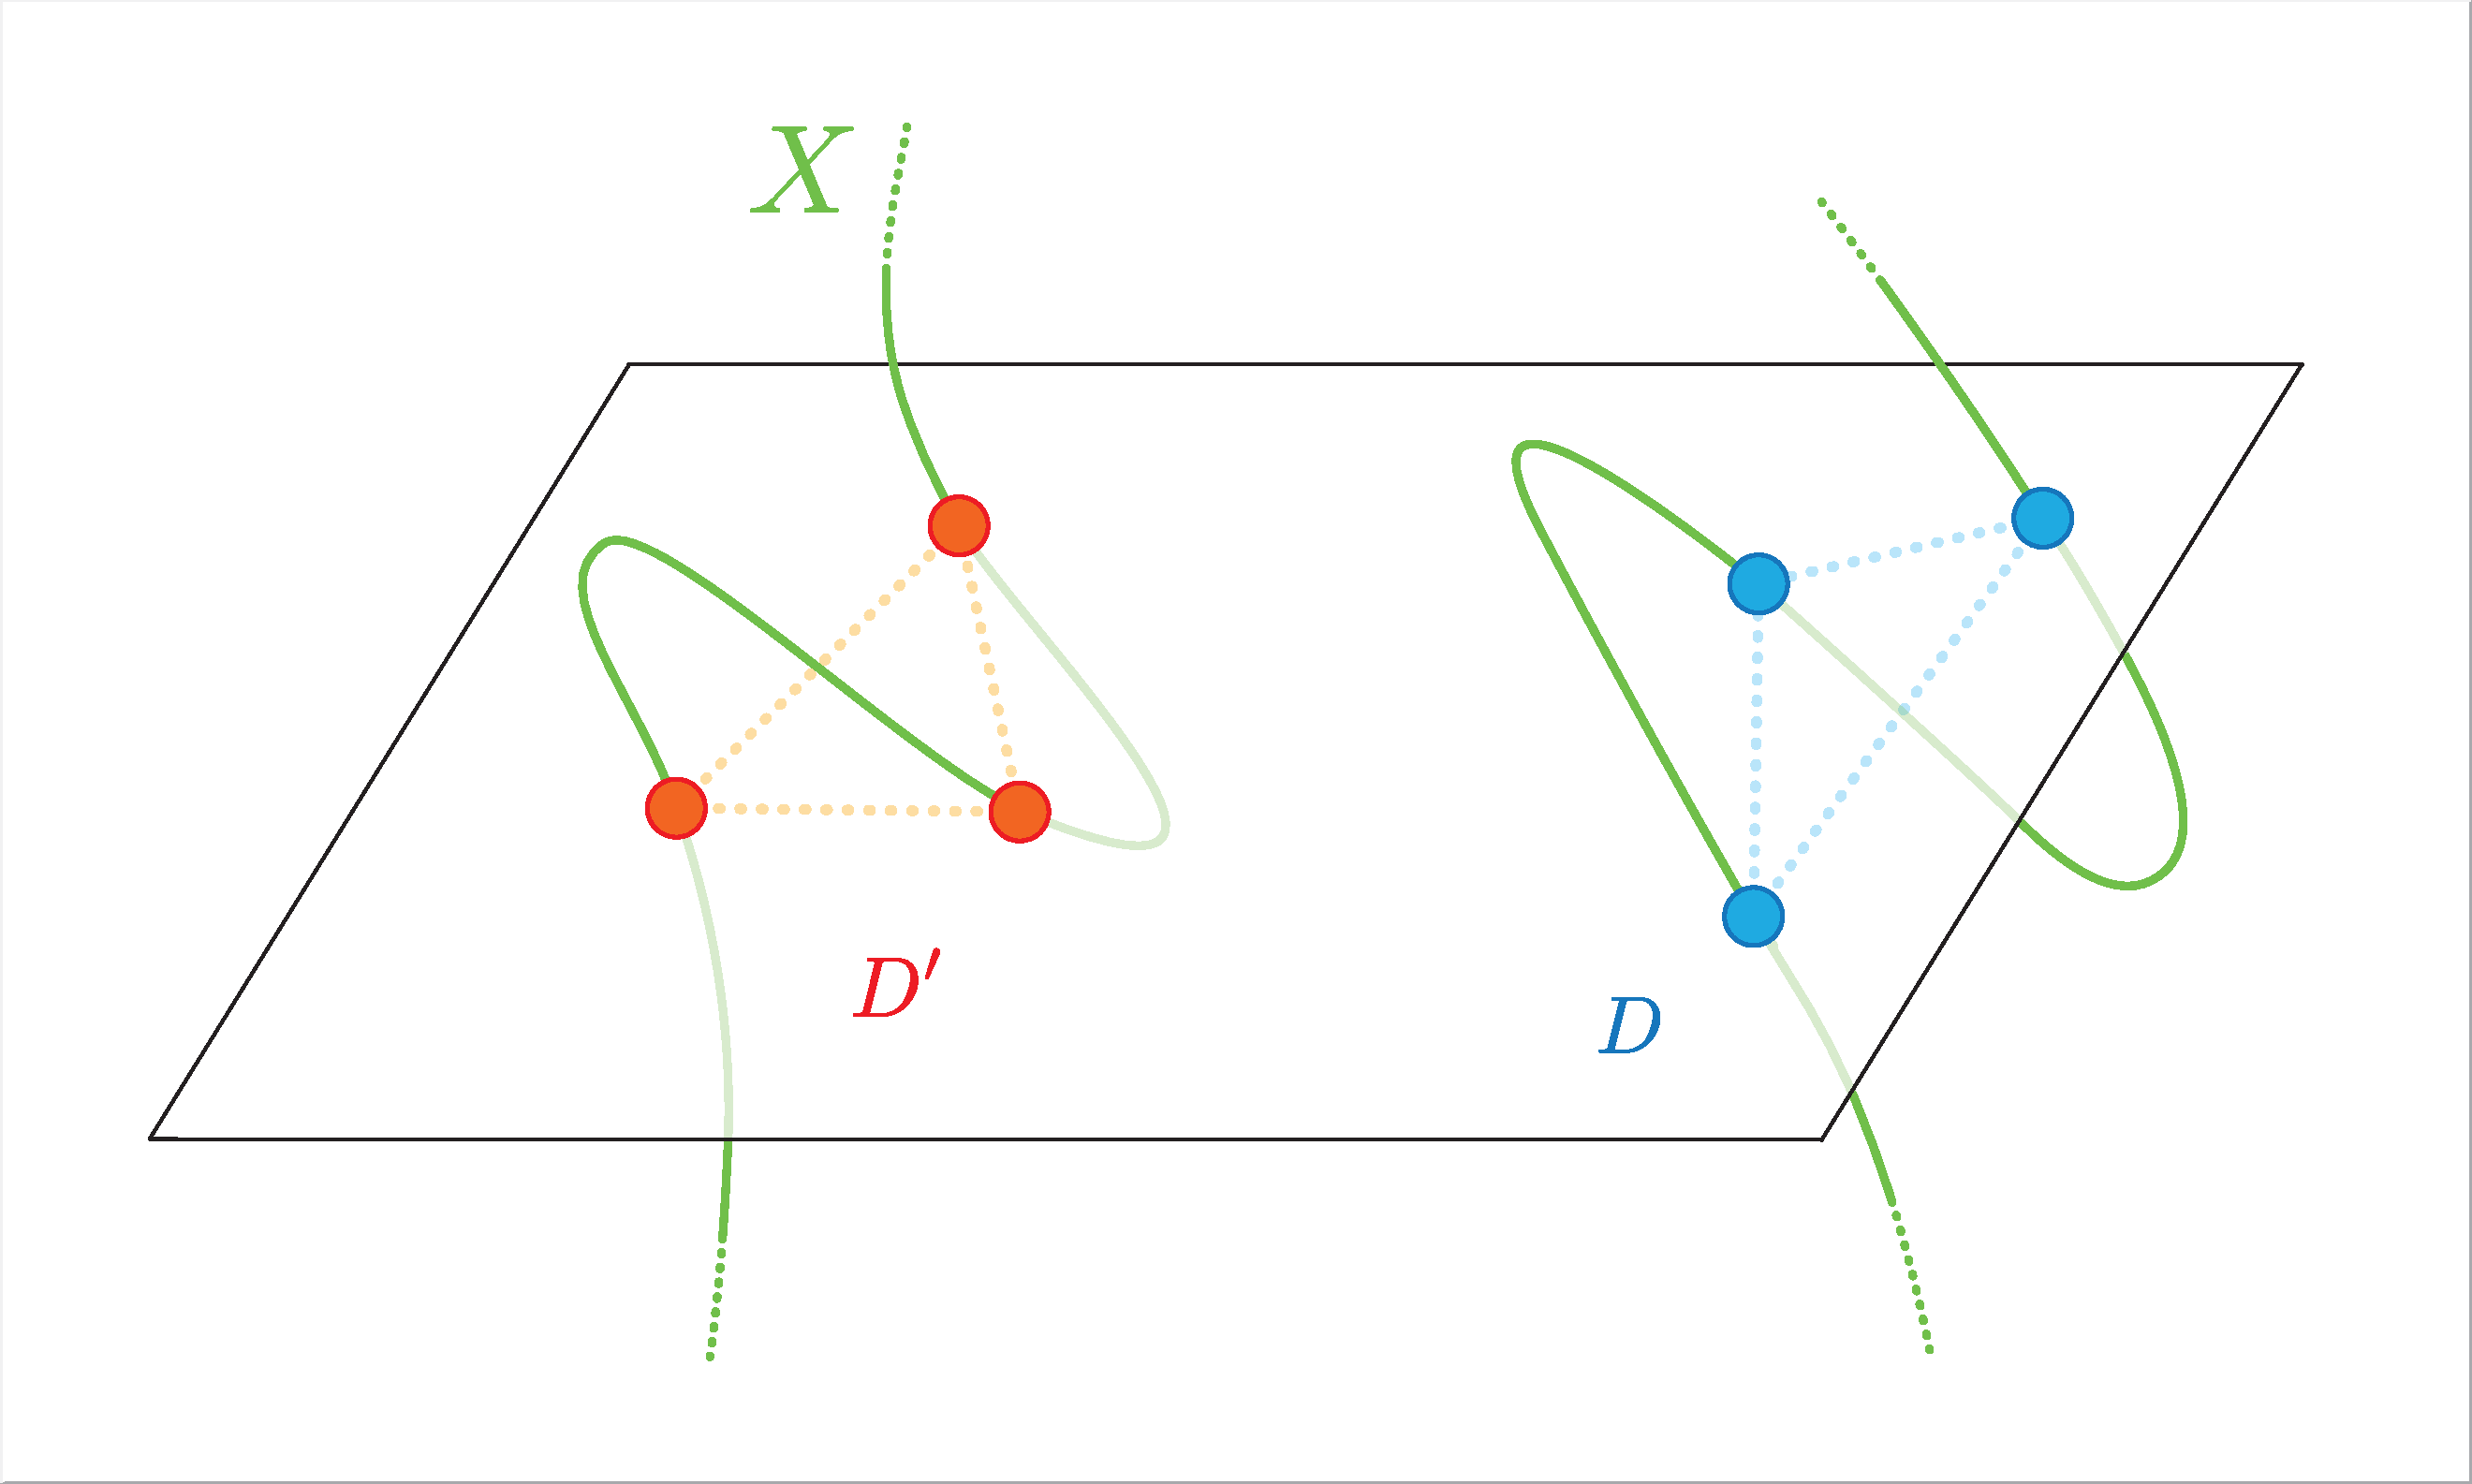
\includegraphics[width=0.85\textwidth]{Example2.pdf}
		\caption{In this example a divisor $D$ of degree $3$ gives rise to a trivial linear series. The reason is that the points of $D'$ are linearly independent, therefore there is only one hyperplane passing through $\phi_K(D+D')$. }
		\label{fig:Example2}
	\end{figure}


\section{Examples}\label{sec:examples}
	
	In this Section we will analyse the case of a non-hyperelliptic curve $X$ of genus $4$ in which, as it follows from the discussion of Section \ref{sec:special}, the only special exceptional linear series -- if any exists -- are $g_1^3$.  
	Actually, the Existence Theorem \ref{thm:existence} states that whenever the \textbf{Brill-Noether number}
	$$ \rho(g,d,r) := g - (r+1)(g-d+r) $$
	is non-negative, then there exists at least one $g_d^r$ on the curve. In our case we find $\rho(4,3,1)=0$ and, as a consequence we deduce that our curve admits a $g_3^1$.\\
	It is a well known fact in algebraic geometry that any smooth projective curve of genus $4$ comes as the complete intersection of a quadric surface with a cubic surface inside $\PP^3$ and, moreover, that any quadric of $\PP^3$ is ( up to projective equivalence ) a ruled surface. Hence we see that there are two distinct possibilities:
	\begin{enumerate}[i)]
		\item If the quadric is smooth, then it is a saddle surface, doubly-ruled by two families of perpendicular lines;
		%In this case there are $2$ distinct $g_3^1$ : one of them cuts on the curve divisors lying on one family of the ruling lines, while the other one  cuts divisors sitting on the perpendicular family -- See Figure \ref{fig:Pringles}
		%
		\item If the quadric is singular, then it is a conic surface and there is only one family of ruling lines, all passing through the singular point. 
		%In this case there is one unique $g_3^1$, and every divisor cut on the curve by the linear series lies on a ruling line passing through the singular point of the quadric -- See Figure \ref{fig:Cone}
 	\end{enumerate}
 	Let us start by looking at the first case of a curve on a smooth quadric surface.

 	\begin{example}\label{ex:smooth_quadric}

 		\begin{figure}[h]
			\centering
			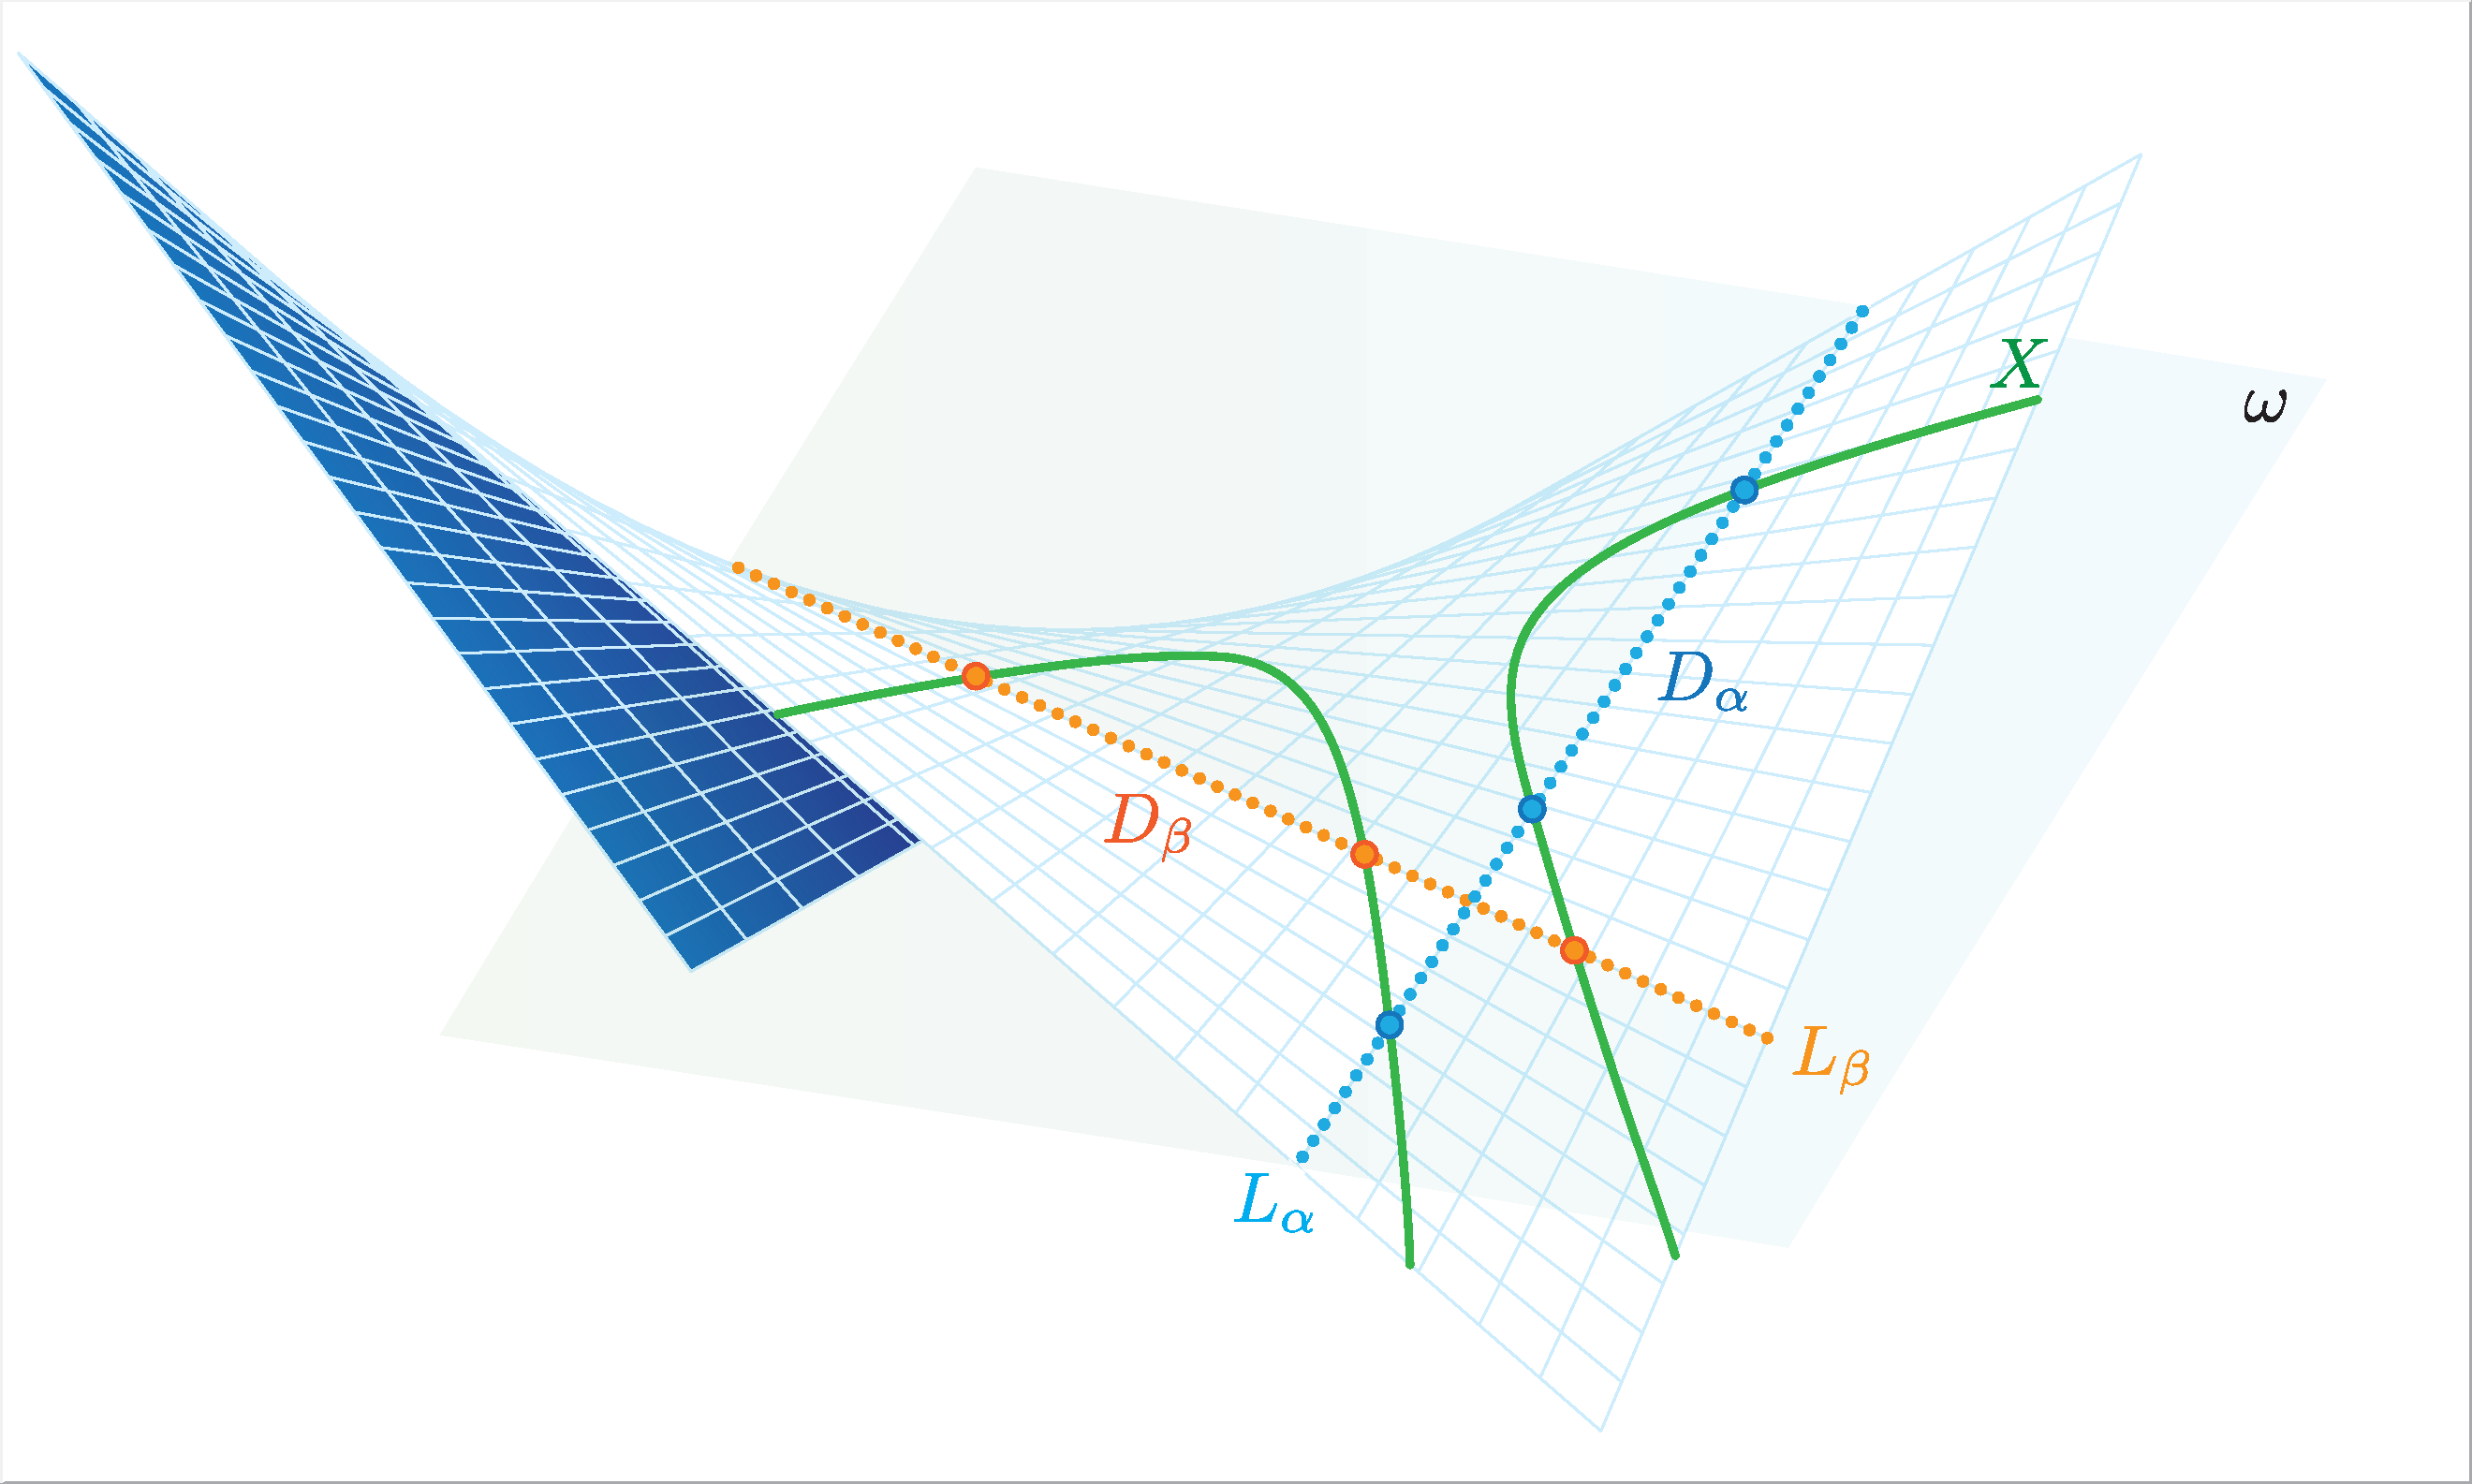
\includegraphics[width=0.85\textwidth]{Pringles2.pdf}
			\caption{ A genus $4$ curve contained in a doubly-ruled smooth quadratic surface -- a hyperbolic paraboloid. The blue dots form the support of a divisor $D_\al$ contained in a $g_3^1$, while the orange ones form the support of the residual $D_\beta$ belonging to the other $g_3^1$ }
			\label{fig:Pringles}
			%\vspace{1em}
		\end{figure}

 		Up to projective equivalence, the smooth quadratic surface $Q$ corresponds to the equation
 		$$ X_0 X_3 = X_1 X_3 $$
 		and it is naturally isomorphic to the product $\PP^1 \times \PP^1$ of two projective lines. The double ruling of $Q$ is given by two $\PP^1$ families of lines
 		$$ A= \begin{cases} X_0=a X_1 \\ X_2=a X_3 \end{cases} \AND B= \begin{cases} X_0=b X_2 \\ X_1=b X_3 \end{cases} $$
 		where the parameters $a$ and $b$ vary in $\PP^1$. It is easy to check that any two lines $L_\al \in A$ and $L_\beta \in B$ intersect in the unique point $[\alb, \beta, \al, 1]$ and, hence, their span is a plane $H_\alb = \Span(L_\al, L_\beta)$. Suppose that such a plane cuts $X$ on the effective divisor
 		$$ H_\alb \cdot X = D_\al + D_\beta, \qquad D_\al\in L_\al, \; D_\beta\in L_\beta $$
 		and recall that, since $H_\alb$ is a hyperplane of $\PP^3$, the divisor $D_\al + D_\beta$ is canonical of degree $2g-2=6$.
 		Each line $L_\al$ and $L_\beta$ moves in a $\PP^1$-family, so it follows that
 		$$ r(D_\al) \geq 1 \AND r(D_\beta) \geq 1 $$
 		and, as a consequence, Clifford's Theorem $\ref{thm:Clifford}$ implies that both $\deg(D_\al)\geq 2$ and $\deg(D_\beta)\geq 2$. But, since $X$ is not hyperelliptic, these inequalities are actually strict and from $\deg(D_\al+D_\beta)=6$ we deduce
 		$ \deg(D_\al) = \deg(D_\beta) = 3 $,
 		thus another application of the Clifford's Theorem ensures that
 		$$ r(D_\al) = r(D_\beta) = 1\,. $$
 		Hence we conclude that the linear series $|D_\al|$ and $|D_\beta|$ are both $g_1^3$ or, in other words, $X$ admits two triple covers of $\PP^1$ obtained by projecting in the directions of $L_\al$ and $L_\beta$. This situation is pictured in Figure $\ref{fig:Example}$, where the orange and the blue lines belong to distinct families of lines and cut a pair of residual divisors.
 	
 	\end{example}

 	\begin{example}\label{ex:singular_quadric}

	 	\begin{figure}[h]
			\centering
			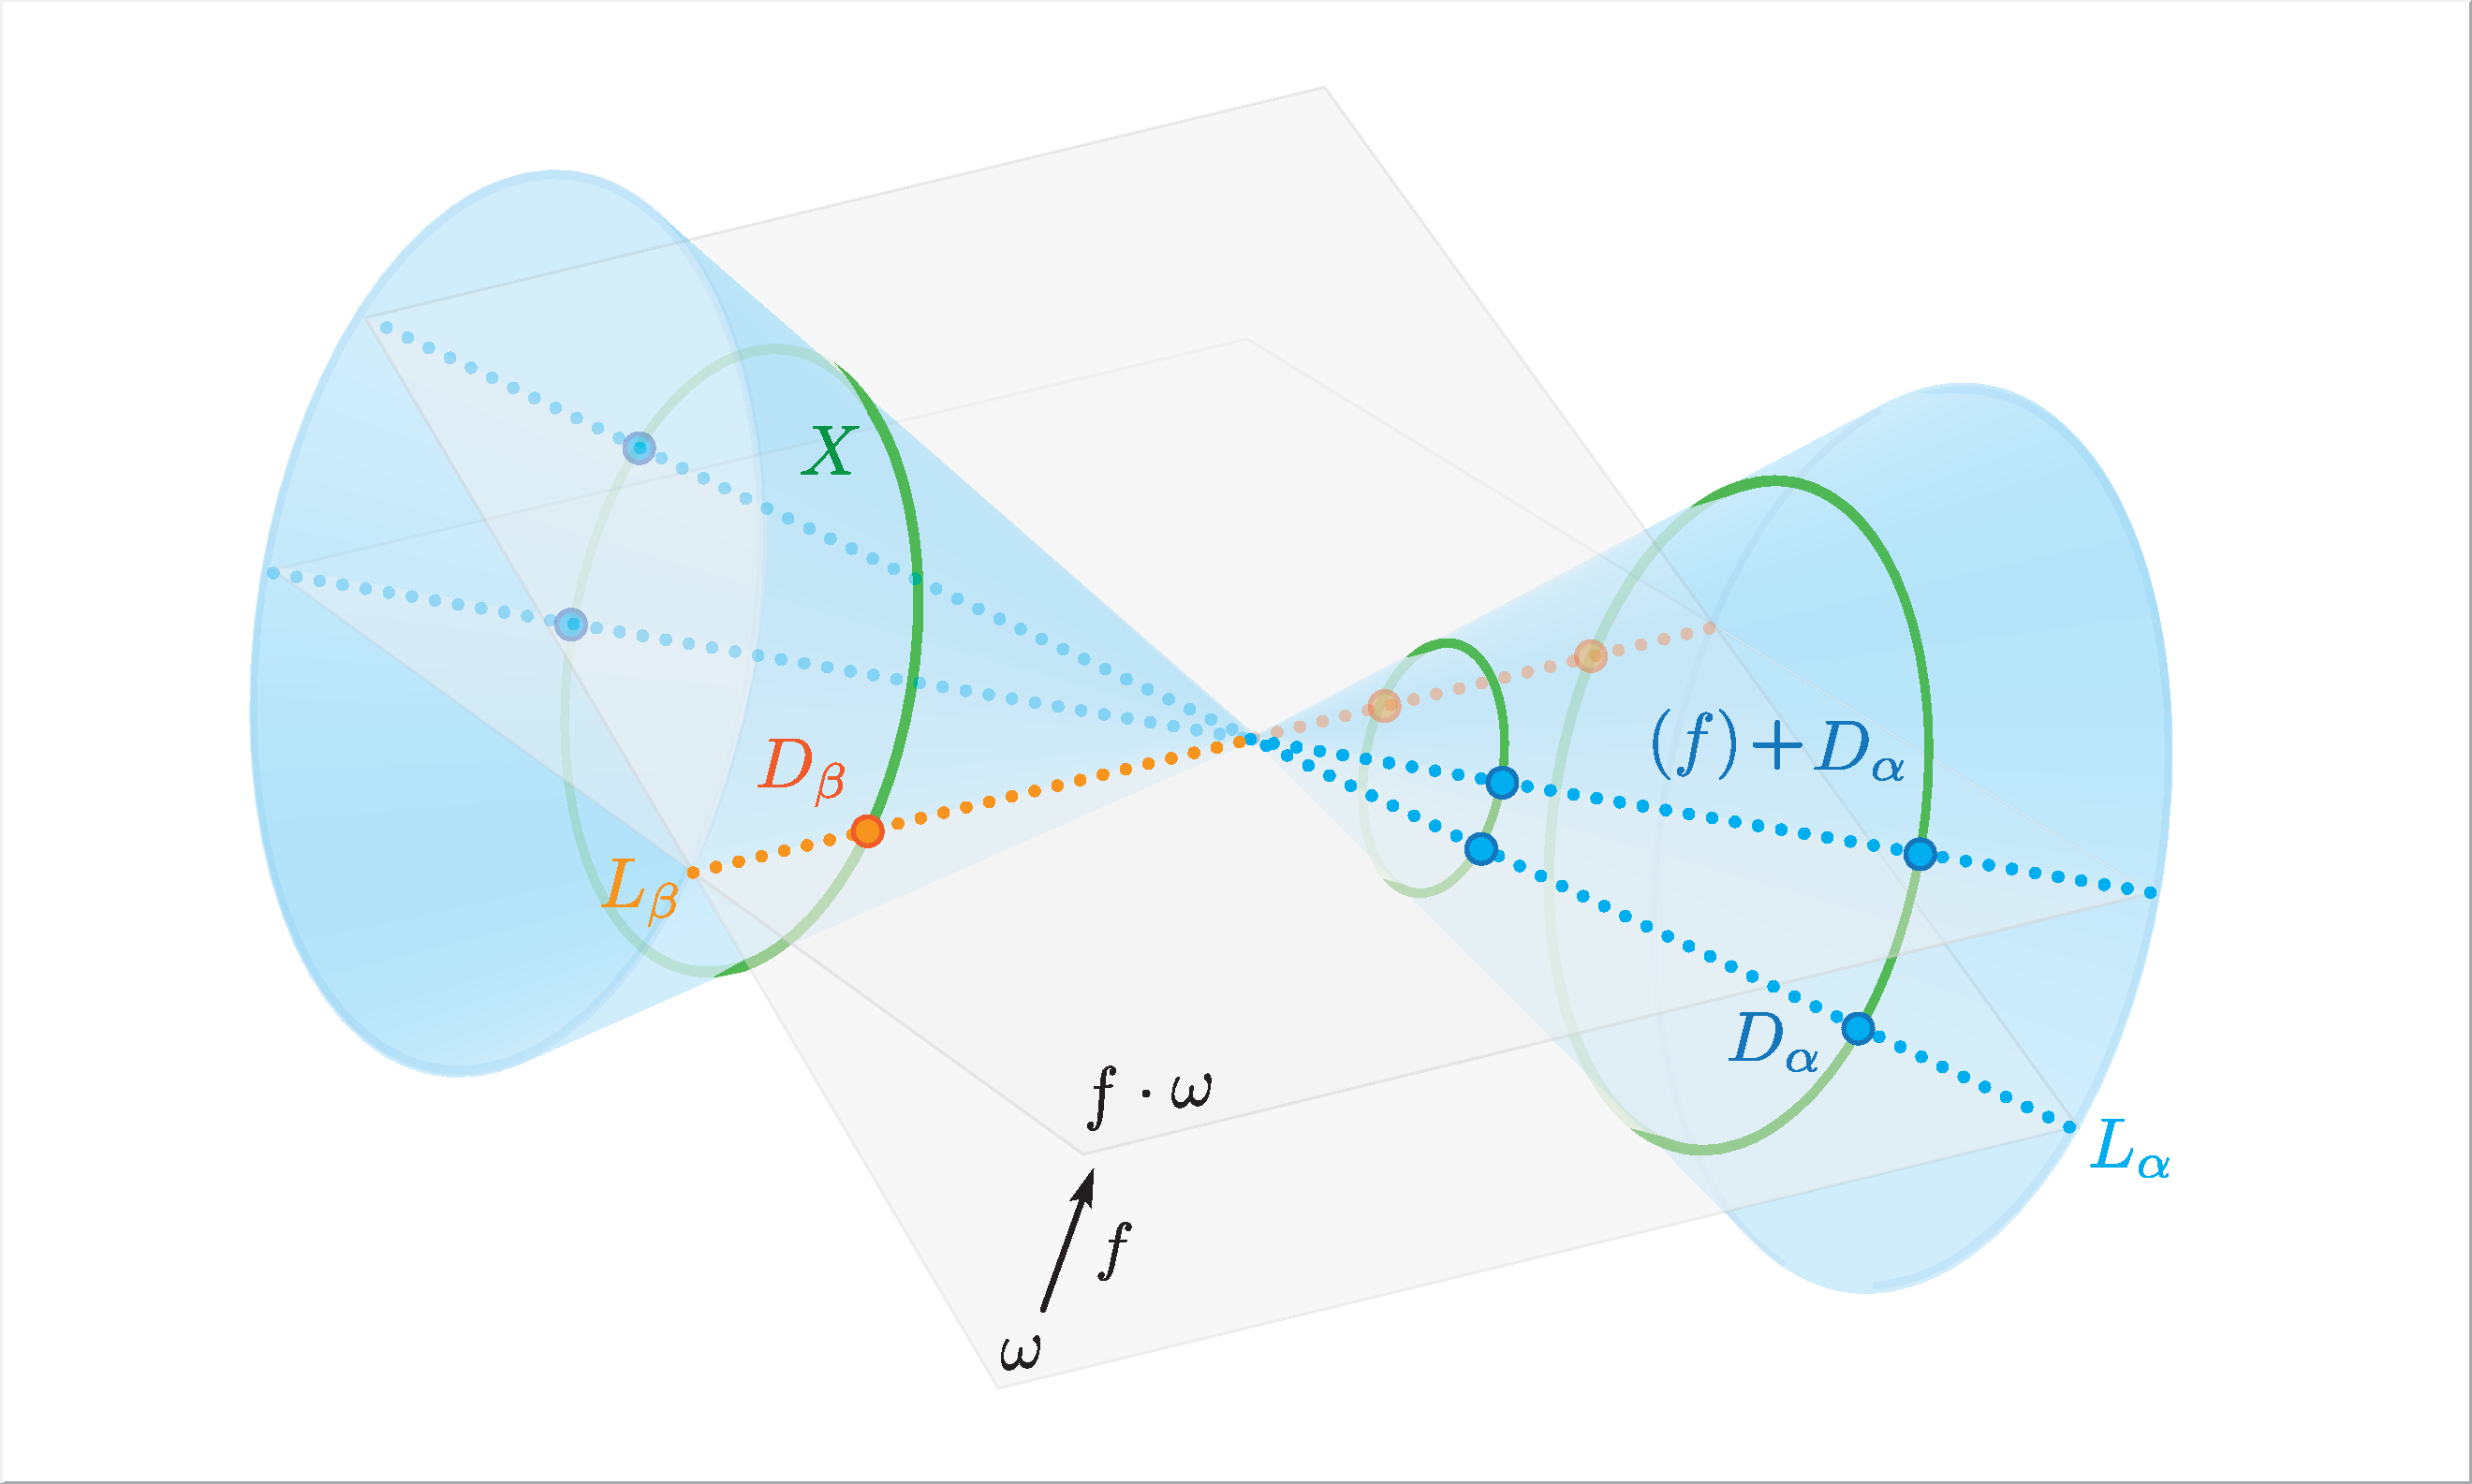
\includegraphics[width=0.85\textwidth]{Cone2.pdf}
			\caption{ A genus $4$ curve contained in a singular ruled quadratic surface -- namely a cone. There is a $\PP^1$-family of hyperplanes passing through $\phi_k(D')$, each one cutting the curve in $D'$ plus a divisor belonging to the unique $g_3^1$. Notice that, in contrast with Figure \ref{fig:Pringles}, every divisor of the $g_3^1$ can be obtained by rotating a plane on the orange axis }
			\label{fig:Cone}
		\end{figure}

		Up to projective equivalence, the singular quadratic surface $Q$ corresponds to the equation
 		$$ X_0^2 = X_1 X_2 $$
 		and can be viewed as the union of a $\PP^1$ family of lines, parametrized by a plane conic, which can be described as
 		$$ A= \begin{cases} X_0=a X_1 \\ X_2=a^2 X_1 \end{cases} $$
 		where the parameter $a$ varies in $\PP^1$. It is easy to check that any two lines $L_\al,\, L_\beta \in A$ intersect in the singular point $[0,0,0,1]$ of $Q$ and, hence, that their span is a plane $H_\alb = \Span(L_\al, L_\beta)$. 
 		Again, such a plane cuts $X$ on the canonical divisor
 		$$ H_\alb \cdot X = D_\al + D_\beta, \qquad D_\al\in L_\al, \; D_\beta\in L_\beta $$
 		and we realize that the situation is closely related to the one of Example \ref{ex:smooth_quadric}. 
 		Reasoning in a similar way one can check that both $D_\al$ and $D_\beta$ give rise to a $g_3^1$, but the crucial difference from the previous Example is that this time there is a unique family of lines and, as a consequence, the two linear series coincide: $|D_\al|=|D_\beta|$.\\
 		The situation is pictured in Figure $\ref{fig:Example2}$, with a $\PP^1$ family of planes \emph{rotating around} $\phi_K(D')$, where each plane intersects the curve in a set of points consisting of $D'$ and a divisor in $|D|$. The reader should notice that a rotation of $H_\w$ by $90$ degrees gives a plane which is tangent to the cone $Q$ and which cuts $X$ in the divisor $2D'$, thus showing that also $D'$ belongs to the linear series $|D|$.

 	
 	\end{example}

 	We therefore see that, in the case of a genus $4$ curve, it is sufficient to count the number of $g_3^1$'s to be able to distinguish between the two possible scenarios described above. More precisely, the variety $G_3^1$ parametrizing linear series of degree $3$ and dimension $1$ is zero dimensional in both cases, but in Example $\ref{ex:smooth_quadric}$ it consists of $2$ distinct points, while it \emph{degenerates} to a unique point in the case of Example $\ref{ex:singular_quadric}$.\\

 	For higher genus the situation becomes more complicated, but still there are many examples in which an analysis of the behaviour of special linear series gives valuable information on the nature of the curve.
	

% ----------------------------------------------------------------------



